\documentclass[10pt,aspectratio=169]{beamer}

\usetheme{Madrid}
\usecolortheme{default}
\usefonttheme{professionalfonts}

\usepackage[utf8]{inputenc}
\usepackage[T1]{fontenc}
\usepackage{lmodern}
\usepackage{amsmath}
\usepackage{booktabs}
\usepackage{array}
\usepackage{tikz}
\usepackage{listings}
\usepackage{xcolor}
\usepackage{multicol}
\usepackage{graphicx}

\usetikzlibrary{arrows.meta,positioning,shapes.geometric,calc,decorations.pathreplacing}

% -------------------------------------------------------------------
% Custom theme
% -------------------------------------------------------------------
\definecolor{SGBlue}{HTML}{0B2545}
\definecolor{SGCyan}{HTML}{2CA6A4}
\definecolor{SGOrange}{HTML}{F28C28}
\definecolor{SGGreen}{HTML}{3A7D44}
\definecolor{SGRed}{HTML}{B23A48}
\definecolor{SGGray}{HTML}{F3F6F8}
\definecolor{SGInk}{HTML}{13202C}
\definecolor{SGLightInk}{HTML}{4A5A66}

\setbeamercolor{normal text}{fg=SGInk,bg=white}
\setbeamercolor{structure}{fg=SGBlue}
\setbeamercolor{frametitle}{fg=white,bg=SGBlue}
\setbeamercolor{title}{fg=white,bg=SGBlue}
\setbeamercolor{subtitle}{fg=white}
\setbeamercolor{block title}{fg=white,bg=SGBlue}
\setbeamercolor{block body}{fg=SGInk,bg=SGGray}
\setbeamercolor{block title alerted}{fg=white,bg=SGRed}
\setbeamercolor{block body alerted}{fg=SGInk,bg=SGGray}
\setbeamercolor{block title example}{fg=white,bg=SGGreen}
\setbeamercolor{block body example}{fg=SGInk,bg=SGGray}

\setbeamertemplate{navigation symbols}{}
\setbeamertemplate{itemize item}{\color{SGCyan}$\blacktriangleright$}
\setbeamertemplate{itemize subitem}{\color{SGOrange}$\bullet$}

\setbeamertemplate{footline}{
  \leavevmode%
  \hbox{%
    \begin{beamercolorbox}[wd=.77\paperwidth,ht=2.6ex,dp=1.2ex,leftskip=1.2em]{author in head/foot}%
      \color{white}\scriptsize SGSMA 2026 final method tutorial
    \end{beamercolorbox}%
    \begin{beamercolorbox}[wd=.23\paperwidth,ht=2.6ex,dp=1.2ex,rightskip=1.2em plus1fil]{date in head/foot}%
      \color{white}\scriptsize \insertframenumber/\inserttotalframenumber
    \end{beamercolorbox}%
  }%
}
\setbeamercolor{author in head/foot}{bg=SGBlue}
\setbeamercolor{date in head/foot}{bg=SGCyan}

\lstdefinestyle{sgcode}{
  basicstyle=\ttfamily\scriptsize,
  keywordstyle=\color{SGBlue}\bfseries,
  commentstyle=\color{SGLightInk},
  stringstyle=\color{SGGreen},
  breaklines=true,
  columns=fullflexible,
  keepspaces=true,
  frame=single,
  rulecolor=\color{SGGray},
  backgroundcolor=\color{SGGray},
  showstringspaces=false
}
\lstset{style=sgcode}

\newcommand{\metric}[2]{%
  \begin{tabular}{@{}c@{}}\Large\bfseries #1\\[-1mm]\scriptsize #2\end{tabular}}
\newcommand{\code}[1]{\texttt{\footnotesize #1}}
\newcommand{\phasebox}[2]{%
  \begin{tikzpicture}[baseline=(n.base)]
    \node[rounded corners=2pt,fill=#1!12,draw=#1,inner xsep=5pt,inner ysep=2pt] (n) {\scriptsize #2};
  \end{tikzpicture}}

\title[SGMS final]{Tutorial paso a paso: metodo final SGSMA}
\subtitle{Deteccion, clasificacion y localizacion de eventos PMU con features fisicas + ExtraTrees}
\author{SGSMA26 Physics-Informed AD}
\date{Presentacion hands-on de 30 minutos}

\begin{document}

% -------------------------------------------------------------------
\begin{frame}[plain,noframenumbering]
  \begin{tikzpicture}[remember picture,overlay]
    \fill[SGBlue] (current page.south west) rectangle (current page.north east);
    \fill[SGCyan] ($(current page.north east)+(-5.4,0)$) -- (current page.north east) -- (current page.south east) -- ($(current page.south east)+(-2.1,0)$) -- cycle;
    \fill[SGOrange] ($(current page.south west)+(0,0)$) rectangle ($(current page.south west)+(1.1,9)$);
  \end{tikzpicture}
  \vspace{1.2cm}
  {\color{white}\Huge\bfseries Tutorial paso a paso}\\[2mm]
  {\color{white}\Large Metodo final enviado al SGSMA Challenge}\\[8mm]
  {\color{white}\large Physics-informed PMU event detection and localization}\\[12mm]
  \begin{block}{}
    \centering
    \textbf{Modelo final:} \code{sgms\_extra\_trees\_windowed\_v2}\\
    \textbf{Variante:} \code{base\_v2 + rolling + rls\_kalman + graph\_temporal}
  \end{block}
\end{frame}

% -------------------------------------------------------------------
\begin{frame}{Mapa de 30 minutos}
\small
\begin{columns}[T,totalwidth=\textwidth]
\begin{column}{0.48\textwidth}
\begin{block}{Parte 1: problema y datos}
\begin{itemize}
  \item Que entra y que debe salir.
  \item Eventos 0--8.
  \item Por que usamos ventanas.
\end{itemize}
\end{block}
\begin{block}{Parte 2: features fisicas}
\begin{itemize}
  \item Baseline pre-evento.
  \item Estadisticas, derivadas, z robusto.
  \item Calidad de datos, bad data y potencia proxy.
\end{itemize}
\end{block}
\end{column}
\begin{column}{0.48\textwidth}
\begin{block}{Parte 3: dinamica y ML}
\begin{itemize}
  \item Rolling, RLS/Kalman y graph temporal.
  \item ExtraTrees jerarquico.
  \item Reglas fisicas de proteccion.
\end{itemize}
\end{block}
\begin{block}{Parte 4: localizacion y resultado}
\begin{itemize}
  \item Localizadores BUS, LINE y PMU.
  \item Pipeline final de inferencia.
  \item Resultados y receta para reprogramar.
\end{itemize}
\end{block}
\end{column}
\end{columns}
\end{frame}

% -------------------------------------------------------------------
\section{Problema}

\begin{frame}{Objetivo del challenge}
\small
\begin{columns}[T,totalwidth=\textwidth]
\begin{column}{0.48\textwidth}
\begin{block}{Entrada}
Series temporales PMU por bus observado:
\begin{itemize}
  \item Voltajes y corrientes trifasicas.
  \item Angulos de tension y corriente.
  \item Frecuencia y ROCOF.
  \item Calidad de datos.
\end{itemize}
\end{block}
\end{column}
\begin{column}{0.48\textwidth}
\begin{block}{Salida requerida}
Archivo CSV con:
\begin{itemize}
  \item \code{TIMESTAMP}
  \item \code{Bus}
  \item \code{Predicted\_Event}
  \item \code{Predicted\_Location}
\end{itemize}
\end{block}
\end{column}
\end{columns}
\vspace{2mm}
\begin{alertblock}{Tarea real}
No basta detectar anomalia. Hay que decidir \textbf{que evento ocurrio} y \textbf{donde ocurrio}: bus, linea o PMU.
\end{alertblock}
\end{frame}

% -------------------------------------------------------------------
\begin{frame}{Eventos que predice el metodo}
\small
\centering
\begin{tabular}{clp{0.54\textwidth}}
\toprule
\textbf{Label} & \textbf{Evento} & \textbf{Lectura fisica principal}\\
\midrule
0 & normal & Sin perturbacion ni problema de datos.\\
1 & fault & Cambio brusco de voltaje, alta derivada, sag/transitorio.\\
2 & line outage & Redistribucion de corriente, sin caida extrema de voltaje.\\
3 & generation change & Cambio de frecuencia, ROCOF y potencia activa proxy.\\
4 & load change & Cambio sostenido de corriente/potencia consumida.\\
5 & missing data & Datos faltantes sin evidencia fisica fuerte.\\
6 & missing + physical & Missing simultaneo con evento fisico.\\
7 & bad data & Una senal aislada se vuelve incoherente.\\
8 & mixed proxy & Firma fisica mixta/no limpia.\\
\bottomrule
\end{tabular}
\end{frame}

% -------------------------------------------------------------------
\begin{frame}{Senales disponibles}
\small
\begin{columns}[T,totalwidth=\textwidth]
\begin{column}{0.50\textwidth}
\begin{block}{Senales electricas}
\begin{tabular}{ll}
\toprule
Grupo & Columnas\\
\midrule
Voltaje mag. & \code{VA\_MAG, VB\_MAG, VC\_MAG}\\
Corriente mag. & \code{IA\_MAG, IB\_MAG, IC\_MAG}\\
Voltaje ang. & \code{VA\_ANG, VB\_ANG, VC\_ANG}\\
Corriente ang. & \code{IA\_ANG, IB\_ANG, IC\_ANG}\\
Dinamica & \code{Freq, ROCOF}\\
\bottomrule
\end{tabular}
\end{block}
\end{column}
\begin{column}{0.46\textwidth}
\begin{block}{Senales de soporte}
\begin{itemize}
  \item \code{TIMESTAMP}
  \item \code{DATA\_PRESENT}
  \item Nombre del archivo \code{Bus*.csv}
  \item Topologia IEEE 39 para distancias electricas.
\end{itemize}
\end{block}
\begin{exampleblock}{Idea clave}
Cada columna se transforma en una evidencia fisica: severidad, rapidez, persistencia, calidad y propagacion espacial.
\end{exampleblock}
\end{column}
\end{columns}
\end{frame}

% -------------------------------------------------------------------
\begin{frame}{Pipeline final en una sola imagen}
\centering
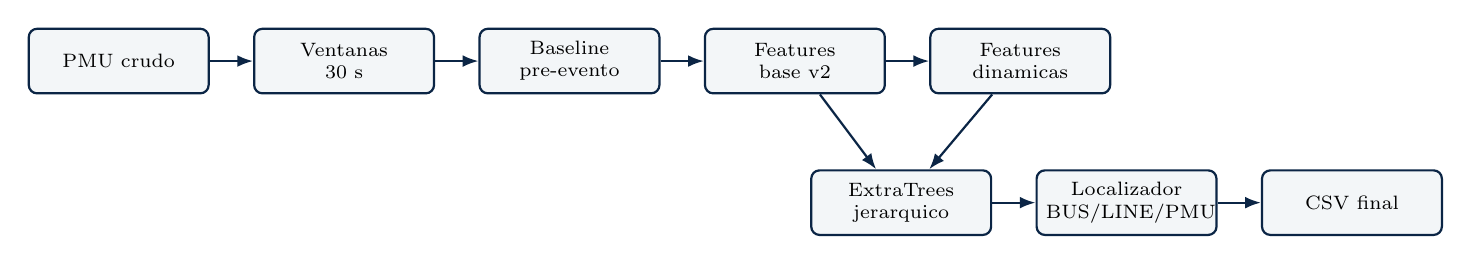
\begin{tikzpicture}[
  node distance=0.9cm and 0.55cm,
  box/.style={rounded corners=3pt,draw=SGBlue,fill=SGGray,thick,minimum height=0.82cm,text width=2.05cm,align=center,font=\scriptsize},
  arrow/.style={-{Latex[length=2mm]},thick,draw=SGBlue}
]
\node[box] (raw) {PMU crudo};
\node[box,right=of raw] (win) {Ventanas\\30 s};
\node[box,right=of win] (base) {Baseline\\pre-evento};
\node[box,right=of base] (feat) {Features\\base v2};
\node[box,right=of feat] (dyn) {Features\\dinamicas};
\node[box,below=0.95cm of feat,xshift=1.35cm] (clf) {ExtraTrees\\jerarquico};
\node[box,right=of clf] (loc) {Localizador\\BUS/LINE/PMU};
\node[box,right=of loc] (out) {CSV final};
\draw[arrow] (raw) -- (win);
\draw[arrow] (win) -- (base);
\draw[arrow] (base) -- (feat);
\draw[arrow] (feat) -- (dyn);
\draw[arrow] (feat) -- (clf);
\draw[arrow] (dyn) -- (clf);
\draw[arrow] (clf) -- (loc);
\draw[arrow] (loc) -- (out);
\end{tikzpicture}
\vspace{4mm}
\begin{block}{Principio del metodo}
El modelo no memoriza la senal cruda. Primero convierte cada ventana en una firma fisica y despues usa ML robusto para decidir evento y localizacion.
\end{block}
\end{frame}

% -------------------------------------------------------------------
\section{Ventanas y baseline}

\begin{frame}{Unidad de decision: ventana de 30 segundos}
\small
\begin{columns}[T,totalwidth=\textwidth]
\begin{column}{0.52\textwidth}
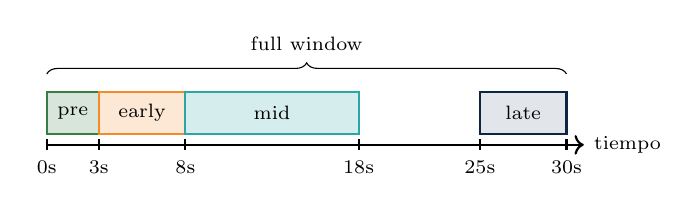
\begin{tikzpicture}[x=0.22cm,y=0.9cm]
  \draw[->,thick] (0,0) -- (31,0) node[right]{\scriptsize tiempo};
  \foreach \x/\txt in {0/0s,3/3s,8/8s,18/18s,25/25s,30/30s} {
    \draw[thick] (\x,0.08) -- (\x,-0.08) node[below]{\scriptsize \txt};
  }
  \fill[SGGreen!20] (0,0.15) rectangle (3,0.75);
  \fill[SGOrange!20] (3,0.15) rectangle (8,0.75);
  \fill[SGCyan!20] (8,0.15) rectangle (18,0.75);
  \fill[SGBlue!12] (25,0.15) rectangle (30,0.75);
  \draw[SGGreen,thick] (0,0.15) rectangle (3,0.75);
  \draw[SGOrange,thick] (3,0.15) rectangle (8,0.75);
  \draw[SGCyan,thick] (8,0.15) rectangle (18,0.75);
  \draw[SGBlue,thick] (25,0.15) rectangle (30,0.75);
  \node at (1.5,0.45) {\scriptsize pre};
  \node at (5.5,0.45) {\scriptsize early};
  \node at (13,0.45) {\scriptsize mid};
  \node at (27.5,0.45) {\scriptsize late};
  \draw[decorate,decoration={brace,amplitude=4pt}] (0,1.0) -- node[above=5pt]{\scriptsize full window} (30,1.0);
\end{tikzpicture}
\end{column}
\begin{column}{0.44\textwidth}
\begin{block}{Por que 30 s}
\begin{itemize}
  \item Captura inicio, transitorio y estado posterior.
  \item Evita decidir con una sola muestra.
  \item Permite generar features estables.
  \item La salida se replica a timestamps de la ventana.
\end{itemize}
\end{block}
\end{column}
\end{columns}
\vspace{2mm}
\begin{exampleblock}{Lectura fisica}
Fault tiende a aparecer en early; cambios de generacion/carga se ven mejor en mid/late; missing se ve como gaps a lo largo de la ventana.
\end{exampleblock}
\end{frame}

% -------------------------------------------------------------------
\begin{frame}{Baseline pre-evento}
\small
\begin{block}{Paso}
Para cada PMU y cada senal, tomar la mediana de los primeros segundos:
\[
  b_x = \mathrm{median}\left(x(t),\ t \in \mathrm{pre}\right)
\]
\end{block}
\begin{columns}[T,totalwidth=\textwidth]
\begin{column}{0.48\textwidth}
\begin{exampleblock}{Magnitudes}
\[
  x_{\mathrm{pu}}(t) = \frac{x(t)}{b_x + \epsilon}
\]
\[
  \Delta x(t) = x(t) - b_x
\]
\end{exampleblock}
\end{column}
\begin{column}{0.48\textwidth}
\begin{alertblock}{Angulos}
Primero se aplica unwrap para no confundir saltos de representacion con eventos reales.
\[
  \theta_{\mathrm{clean}} = \mathrm{unwrap}(\theta)
\]
\end{alertblock}
\end{column}
\end{columns}
\vspace{1mm}
\begin{block}{Por que importa}
Cada PMU se compara contra su propio estado normal. Asi el modelo aprende cambios relativos, no valores absolutos fragiles.
\end{block}
\end{frame}

% -------------------------------------------------------------------
\section{Feature engineering base}

\begin{frame}{Familias de features base v2}
\small
\centering
\begin{tabular}{p{0.25\textwidth}p{0.36\textwidth}p{0.29\textwidth}}
\toprule
\textbf{Familia} & \textbf{Que calcula} & \textbf{Que significa}\\
\midrule
Estadisticas por senal & media, std, min, max, span, percentiles & magnitud y severidad\\
Deltas temporales & early-pre, mid-pre, late-pre & evolucion del evento\\
Derivadas & max derivada, RMS derivada & rapidez/transitorio\\
Robust z-score & desvio contra MAD pre-evento & anomalia relativa\\
Data quality & gaps, NaNs, DATA\_PRESENT & missing o PMU caido\\
Single-signal & max/second/ratio de anomalias & bad data aislado\\
Power proxy & P, Q, angulo de factor de potencia & generacion/carga\\
Agregados globales & mean/max/min/std entre PMUs & patron espacial\\
\bottomrule
\end{tabular}
\end{frame}

% -------------------------------------------------------------------
\begin{frame}{Features estadisticas por senal}
\small
\begin{block}{Se calculan para cada senal y cada segmento}
\[
\{\mathrm{mean},\ \mathrm{std},\ \mathrm{min},\ \mathrm{max},\ \mathrm{span},\ 
\mathrm{median},\ \mathrm{max\_abs},\ \mathrm{mean\_abs},\ p05,\ p95\}
\]
\end{block}
\begin{columns}[T,totalwidth=\textwidth]
\begin{column}{0.48\textwidth}
\begin{exampleblock}{Ejemplo de nombre de feature}
\code{Bus2\_\_VA\_MAG\_\_early\_\_span}\\[1mm]
\code{Bus10\_\_Freq\_\_late\_\_mean}
\end{exampleblock}
\end{column}
\begin{column}{0.48\textwidth}
\begin{block}{Interpretacion}
\begin{itemize}
  \item \textbf{span}: cuanto se movio la senal.
  \item \textbf{std}: oscilacion o inestabilidad.
  \item \textbf{p05/p95}: extremos robustos.
  \item \textbf{mean/median}: cambio de nivel.
\end{itemize}
\end{block}
\end{column}
\end{columns}
\end{frame}

% -------------------------------------------------------------------
\begin{frame}{Deltas temporales y derivadas}
\small
\begin{columns}[T,totalwidth=\textwidth]
\begin{column}{0.50\textwidth}
\begin{block}{Deltas contra pre-evento}
\[
\Delta_{\mathrm{early}} = \mu_{\mathrm{early}} - \mu_{\mathrm{pre}}
\]
\[
\Delta_{\mathrm{mid}} = \mu_{\mathrm{mid}} - \mu_{\mathrm{pre}}
\]
\[
\Delta_{\mathrm{late}} = \mu_{\mathrm{late}} - \mu_{\mathrm{pre}}
\]
\end{block}
\end{column}
\begin{column}{0.46\textwidth}
\begin{block}{Derivadas}
\[
d_x(t) = \frac{x(t)-x(t-\Delta t)}{\Delta t}
\]
\[
\mathrm{max\_abs\_derivative},\quad \mathrm{rms\_derivative}
\]
\end{block}
\end{column}
\end{columns}
\vspace{2mm}
\begin{exampleblock}{Uso por evento}
\begin{itemize}
  \item Fault: derivada alta en voltaje.
  \item Line outage: derivada alta en corriente.
  \item Load/generation: late-pre sostenido.
\end{itemize}
\end{exampleblock}
\end{frame}

% -------------------------------------------------------------------
\begin{frame}{Robust z-score}
\small
\begin{block}{Definicion}
\[
m = \mathrm{median}(x_{\mathrm{pre}})
\]
\[
\mathrm{MAD} = \mathrm{median}(|x_{\mathrm{pre}} - m|)
\]
\[
z_{\mathrm{robust}}(t) = \frac{|x(t)-m|}{\mathrm{MAD}+\epsilon}
\]
\end{block}
\begin{columns}[T,totalwidth=\textwidth]
\begin{column}{0.48\textwidth}
\begin{block}{Features}
\begin{itemize}
  \item \code{max\_abs\_robust\_z}
  \item \code{sustained\_abs\_robust\_z\_5}
  \item \code{sustained\_abs\_robust\_z\_15}
\end{itemize}
\end{block}
\end{column}
\begin{column}{0.48\textwidth}
\begin{exampleblock}{Interpretacion}
Mide que tan rara fue una senal respecto a su propio estado pre-evento. Es mas estable que usar solo media y desviacion estandar.
\end{exampleblock}
\end{column}
\end{columns}
\end{frame}

% -------------------------------------------------------------------
\begin{frame}{Data quality: detectar missing}
\small
\begin{columns}[T,totalwidth=\textwidth]
\begin{column}{0.52\textwidth}
\begin{block}{Features principales}
\begin{itemize}
  \item \code{n\_samples}
  \item \code{dt\_s}, \code{duration\_s}
  \item \code{max\_timestamp\_gap\_s}
  \item \code{max\_timestamp\_gap\_ratio}
  \item \code{data\_present\_fraction}
  \item \code{data\_present\_min}
  \item \code{missing\_run\_max\_s}
  \item \code{nan\_fraction\_max/mean}
\end{itemize}
\end{block}
\end{column}
\begin{column}{0.44\textwidth}
\begin{alertblock}{Decision conceptual}
\[
\mathrm{missing} \Rightarrow
\begin{cases}
\mathrm{Event\ 5}, & \text{si no hay evento fisico}\\
\mathrm{Event\ 6}, & \text{si hay evento fisico}
\end{cases}
\]
\end{alertblock}
\begin{exampleblock}{Senal fisica}
Gaps temporales o DATA\_PRESENT bajo indican falla de medicion/comunicacion, no necesariamente falla electrica.
\end{exampleblock}
\end{column}
\end{columns}
\end{frame}

% -------------------------------------------------------------------
\begin{frame}{Bad data: una senal aislada rompe el patron}
\small
\begin{block}{Features single-signal}
\begin{itemize}
  \item \code{single\_signal\_score\_max}
  \item \code{single\_signal\_score\_second}
  \item \code{single\_signal\_score\_ratio}
  \item \code{single\_signal\_score\_count\_gt20}
\end{itemize}
\end{block}
\begin{columns}[T,totalwidth=\textwidth]
\begin{column}{0.50\textwidth}
\begin{exampleblock}{Intuicion}
Si una sola columna explota y las demas siguen coherentes, probablemente no es un evento electrico global: es dato corrupto.
\end{exampleblock}
\end{column}
\begin{column}{0.46\textwidth}
\begin{alertblock}{Regla mental}
\[
\frac{\mathrm{score}_{1}}{\mathrm{score}_{2}} \geq 3
\quad\Rightarrow\quad
\mathrm{bad\ data\ candidate}
\]
\end{alertblock}
\end{column}
\end{columns}
\end{frame}

% -------------------------------------------------------------------
\begin{frame}{Power proxy: aproximar P y Q sin potencia medida}
\small
\begin{columns}[T,totalwidth=\textwidth]
\begin{column}{0.50\textwidth}
\begin{block}{Por fase}
\[
\phi = \theta_V - \theta_I
\]
\[
P_{\mathrm{proxy}} = V_{\mathrm{pu}} I_{\mathrm{pu}} \cos(\phi)
\]
\[
Q_{\mathrm{proxy}} = V_{\mathrm{pu}} I_{\mathrm{pu}} \sin(\phi)
\]
\[
PF_{\mathrm{ang}} = \phi
\]
\end{block}
\end{column}
\begin{column}{0.46\textwidth}
\begin{exampleblock}{Para que sirve}
\begin{itemize}
  \item Event 3: cambio de generacion.
  \item Event 4: cambio de carga.
  \item Event 8: firma fisica mixta.
\end{itemize}
\end{exampleblock}
\begin{alertblock}{Idea}
Generacion/carga muchas veces se separan mejor por potencia y frecuencia que por voltaje.
\end{alertblock}
\end{column}
\end{columns}
\end{frame}

% -------------------------------------------------------------------
\begin{frame}{Tamano de las features base}
\small
\centering
\begin{tabular}{lr}
\toprule
\textbf{Grupo} & \textbf{Numero aproximado}\\
\midrule
Voltage angle & 7,596\\
Voltage magnitude & 7,596\\
Current angle & 7,596\\
Current magnitude & 7,596\\
Frequency / ROCOF & 4,640\\
Power proxy & 4,428\\
Data quality & 156\\
Single-signal anomaly & 48\\
Other/global & 60\\
\midrule
\textbf{Total base v2} & \textbf{39,716}\\
\bottomrule
\end{tabular}
\vspace{3mm}
\begin{block}{Lectura}
El modelo no ve miles de puntos crudos; ve una firma compacta y fisicamente interpretable de cada ventana.
\end{block}
\end{frame}

% -------------------------------------------------------------------
\section{Features dinamicas}

\begin{frame}{Por que agregar features dinamicas}
\small
\begin{block}{Limitacion de features base}
Las estadisticas resumen \textbf{cuanto} cambio una senal, pero no siempre capturan bien \textbf{como} evoluciono ni \textbf{como se propago} entre PMUs.
\end{block}
\begin{columns}[T,totalwidth=\textwidth]
\begin{column}{0.32\textwidth}
\begin{exampleblock}{Rolling}
Escalas temporales cortas y largas.
\end{exampleblock}
\end{column}
\begin{column}{0.32\textwidth}
\begin{exampleblock}{RLS/Kalman}
Residuo e innovacion contra una dinamica suave.
\end{exampleblock}
\end{column}
\begin{column}{0.32\textwidth}
\begin{exampleblock}{Graph temporal}
Diferencias entre PMUs y tiempo de llegada.
\end{exampleblock}
\end{column}
\end{columns}
\vspace{2mm}
\begin{alertblock}{Variante final}
\code{base\_v2 + rolling + rls\_kalman + graph\_temporal}
\end{alertblock}
\end{frame}

% -------------------------------------------------------------------
\begin{frame}{Bloque rolling}
\small
\begin{columns}[T,totalwidth=\textwidth]
\begin{column}{0.44\textwidth}
\begin{block}{Ventanas internas}
\[
w \in \{5,15,30,60,120\}
\]
Se aplican sobre senales como:
\begin{itemize}
  \item \code{VA\_MAG}, \code{IA\_MAG}
  \item \code{VA\_ANG}, \code{IA\_ANG}
  \item \code{Freq}, \code{ROCOF}
\end{itemize}
\end{block}
\end{column}
\begin{column}{0.52\textwidth}
\begin{block}{Features}
\begin{itemize}
  \item \code{mean\_abs\_max}
  \item \code{std\_max}, \code{std\_mean}
  \item \code{slope\_max\_abs}
  \item \code{energy}
  \item \code{time\_to\_abs\_peak}
\end{itemize}
\end{block}
\begin{exampleblock}{Significado}
Rapidez, energia sostenida y momento del pico. Ayuda a distinguir transitorios bruscos de cambios lentos.
\end{exampleblock}
\end{column}
\end{columns}
\end{frame}

% -------------------------------------------------------------------
\begin{frame}{Bloque RLS/Kalman}
\small
\begin{columns}[T,totalwidth=\textwidth]
\begin{column}{0.50\textwidth}
\begin{block}{Idea}
Un filtro espera que la senal siga una trayectoria suave. Cuando ocurre un evento, el residuo o la innovacion sube.
\end{block}
\begin{block}{Senales usadas}
\code{VA\_MAG, IA\_MAG, VA\_ANG, IA\_ANG, Freq, ROCOF}
\end{block}
\end{column}
\begin{column}{0.46\textwidth}
\begin{block}{Features}
\begin{itemize}
  \item \code{level\_resid}
  \item \code{theta\_delta}
  \item \code{linear\_resid}
  \item \code{kalman\_innov}
  \item max, mean, p95, late-pre, time-to-peak
\end{itemize}
\end{block}
\end{column}
\end{columns}
\vspace{2mm}
\begin{exampleblock}{Lectura fisica}
Si el cambio no se explica por tendencia normal, es evidencia de evento dinamico real.
\end{exampleblock}
\end{frame}

% -------------------------------------------------------------------
\begin{frame}{Bloque graph temporal}
\small
\begin{columns}[T,totalwidth=\textwidth]
\begin{column}{0.52\textwidth}
\begin{block}{Que compara}
\begin{itemize}
  \item Spread entre PMUs.
  \item Diferencias por pares de PMUs.
  \item Correlaciones por pares.
  \item Diferencias en tiempo al pico.
  \item Diferencias ponderadas por distancia electrica.
\end{itemize}
\end{block}
\end{column}
\begin{column}{0.44\textwidth}
\begin{exampleblock}{Por que localiza}
Un evento cerca de un bus o linea afecta mas fuerte y antes a ciertos PMUs. El patron espacial ayuda a inferir el origen.
\end{exampleblock}
\begin{alertblock}{Features clave}
\code{time\_to\_peak\_range}\\
\code{pair\_diff}\\
\code{pair\_corr}\\
\code{weighted\_graph\_diff}
\end{alertblock}
\end{column}
\end{columns}
\end{frame}

% -------------------------------------------------------------------
\begin{frame}{Feature vector final}
\small
\begin{columns}[T,totalwidth=\textwidth]
\begin{column}{0.45\textwidth}
\begin{block}{Base}
\[
n_{\mathrm{base}} \approx 39{,}716
\]
\begin{itemize}
  \item Senales fisicas.
  \item Calidad de datos.
  \item Potencia proxy.
  \item Agregados globales.
\end{itemize}
\end{block}
\end{column}
\begin{column}{0.51\textwidth}
\begin{alertblock}{Final localizer}
\[
n_{\mathrm{final}} = 45{,}162
\]
\begin{itemize}
  \item \code{base\_v2}
  \item \code{rolling}
  \item \code{rls\_kalman}
  \item \code{graph\_temporal}
\end{itemize}
\end{alertblock}
\end{column}
\end{columns}
\vspace{2mm}
\begin{exampleblock}{Decision final}
Se escogio esta variante porque logro el mejor RAW localization entre variantes productivas, manteniendo buen nivel en SIM.
\end{exampleblock}
\end{frame}

% -------------------------------------------------------------------
\section{Modelos}

\begin{frame}{Modelo ML: SimpleImputer + ExtraTrees}
\small
\begin{columns}[T,totalwidth=\textwidth]
\begin{column}{0.46\textwidth}
\begin{block}{Pipeline de cada modelo}
\[
\mathrm{features}
\rightarrow
\mathrm{median\ imputer}
\rightarrow
\mathrm{ExtraTreesClassifier}
\]
\end{block}
\begin{block}{Por que imputar}
Algunas ventanas pueden tener NaNs o columnas faltantes por problemas de datos. La mediana es simple y estable.
\end{block}
\end{column}
\begin{column}{0.50\textwidth}
\begin{exampleblock}{Por que ExtraTrees}
\begin{itemize}
  \item Maneja decenas de miles de features.
  \item No necesita escalado.
  \item Captura no-linealidad.
  \item Es robusto a outliers.
  \item Entrena rapido y sirve con datos mixtos.
\end{itemize}
\end{exampleblock}
\end{column}
\end{columns}
\end{frame}

% -------------------------------------------------------------------
\begin{frame}{Arquitectura jerarquica}
\small
\centering
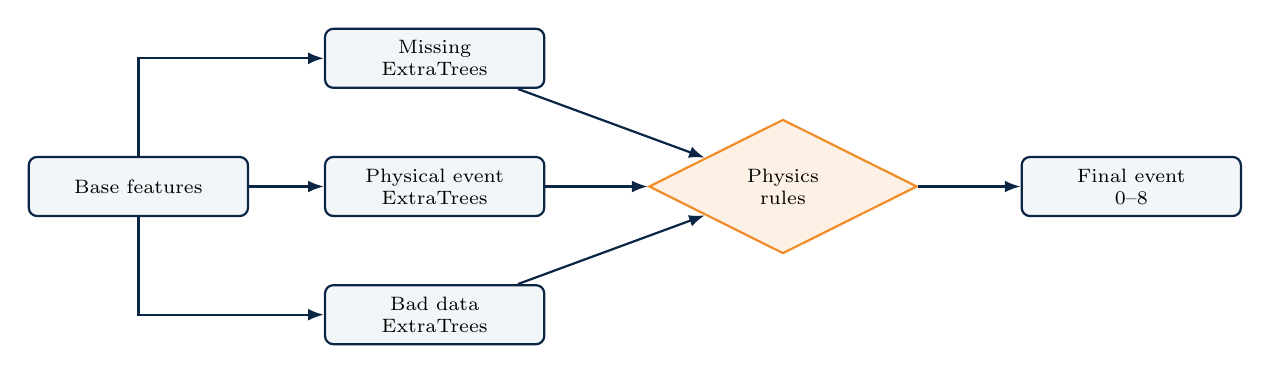
\begin{tikzpicture}[
  node distance=0.85cm and 0.95cm,
  box/.style={rounded corners=3pt,draw=SGBlue,fill=SGGray,thick,minimum height=0.75cm,text width=2.55cm,align=center,font=\scriptsize},
  gate/.style={diamond,aspect=2,draw=SGOrange,fill=SGOrange!12,thick,text width=1.8cm,align=center,font=\scriptsize},
  arrow/.style={-{Latex[length=2mm]},thick,draw=SGBlue}
]
\node[box] (x) {Base features};
\node[box,right=of x] (phys) {Physical event\\ExtraTrees};
\node[box,below=of phys] (bad) {Bad data\\ExtraTrees};
\node[box,above=of phys] (miss) {Missing\\ExtraTrees};
\node[gate,right=1.3cm of phys] (rules) {Physics\\rules};
\node[box,right=1.3cm of rules] (event) {Final event\\0--8};
\draw[arrow] (x) -- (phys);
\draw[arrow] (x) |- (bad);
\draw[arrow] (x) |- (miss);
\draw[arrow] (phys) -- (rules);
\draw[arrow] (bad) -- (rules);
\draw[arrow] (miss) -- (rules);
\draw[arrow] (rules) -- (event);
\end{tikzpicture}
\vspace{4mm}
\begin{block}{No usamos un unico clasificador plano}
Primero se predicen eventos fisicos principales; despues missing y bad data corrigen o reemplazan la decision usando reglas fisicas.
\end{block}
\end{frame}

% -------------------------------------------------------------------
\begin{frame}{Modelos finales entrenados}
\small
\centering
\begin{tabular}{p{0.29\textwidth}p{0.31\textwidth}p{0.28\textwidth}}
\toprule
\textbf{Artefacto} & \textbf{Rol} & \textbf{Clases/Salida}\\
\midrule
\code{physical\_event\_classifier} & Clasificador fisico principal & 0, 1, 2, 3, 4, 8\\
\code{bad\_data\_detector} & Detecta Event 7 & bad/no bad\\
\code{missing\_composition\_detector} & Decide missing puro vs compuesto & missing/no missing\\
\code{final\_dynamic\_localizers} & Localizadores tipados & BUS, LINE, PMU\\
\bottomrule
\end{tabular}
\vspace{3mm}
\begin{exampleblock}{Ruta runtime}
\code{main.py} $\rightarrow$ \code{src/models/hybrid\_submission.py} $\rightarrow$ \code{src/data\_factory/final\_model.py}
\end{exampleblock}
\end{frame}

% -------------------------------------------------------------------
\begin{frame}{Reglas fisicas que protegen el clasificador}
\small
\begin{columns}[T,totalwidth=\textwidth]
\begin{column}{0.50\textwidth}
\begin{block}{Fault-like}
\[
V_{\mathrm{span}} \geq 50000
\]
\[
\mathrm{max}|dV/dt| \geq 500000
\]
\end{block}
\begin{block}{Line-outage-like}
\[
I_{\mathrm{span}} \geq 500
\]
\[
\mathrm{max}|dI/dt| \geq 3000
\]
\[
V_{\mathrm{span}} \leq 50000
\]
\end{block}
\end{column}
\begin{column}{0.46\textwidth}
\begin{alertblock}{Missing-like}
\[
\mathrm{DATA\_PRESENT} < 0.999
\]
o NaNs/gaps altos.
\end{alertblock}
\begin{alertblock}{Bad-data-like}
\[
\mathrm{single\_signal\_score}\ \text{alto}
\]
\[
\mathrm{single\_signal\_ratio} \geq 3
\]
\end{alertblock}
\end{column}
\end{columns}
\end{frame}

% -------------------------------------------------------------------
\begin{frame}{Logica final de evento}
\small
\begin{block}{Orden conceptual}
\begin{enumerate}
  \item Predecir evento fisico con ExtraTrees: 0,1,2,3,4,8.
  \item Medir si hay missing.
  \item Medir si hay bad data.
  \item Aplicar reglas de fault/line/missing/bad.
  \item Emitir evento final 0--8.
\end{enumerate}
\end{block}
\begin{exampleblock}{Traduccion practica}
\begin{itemize}
  \item Missing sin fisica fuerte $\rightarrow$ Event 5.
  \item Missing con fisica fuerte $\rightarrow$ Event 6.
  \item Una senal aislada absurda $\rightarrow$ Event 7.
  \item Voltaje brutal $\rightarrow$ Event 1.
  \item Corriente fuerte sin sag brutal $\rightarrow$ Event 2.
\end{itemize}
\end{exampleblock}
\end{frame}

% -------------------------------------------------------------------
\section{Localizacion}

\begin{frame}{Localizacion tipada}
\small
\begin{columns}[T,totalwidth=\textwidth]
\begin{column}{0.48\textwidth}
\begin{block}{Routing evento $\rightarrow$ localizador}
\begin{tabular}{cl}
\toprule
Evento & Localizador\\
\midrule
1 fault & BUS\\
2 line outage & LINE\\
3 generation & BUS\\
4 load & BUS\\
5 missing & PMU\\
6 missing + physical & BUS o LINE\\
7 bad data & PMU\\
8 mixed proxy & BUS\\
\bottomrule
\end{tabular}
\end{block}
\end{column}
\begin{column}{0.48\textwidth}
\begin{exampleblock}{Por que tipado}
No se localiza igual una linea abierta que un PMU con datos malos. Cada tipo de evento tiene geometria y firma fisica diferente.
\end{exampleblock}
\begin{alertblock}{Localizadores finales}
\code{BUS}, \code{BUS:event1}, \code{BUS:event3}, \code{BUS:event4}, \code{BUS:event8}, \code{LINE}, \code{LINE:event2}, \code{PMU}
\end{alertblock}
\end{column}
\end{columns}
\end{frame}

% -------------------------------------------------------------------
\begin{frame}{Como se localiza fisicamente}
\small
\begin{block}{Evidencias que usa el localizador}
\begin{itemize}
  \item Que PMU tuvo mayor severidad.
  \item Que PMU vio primero el pico.
  \item Que pares de PMUs se movieron juntos.
  \item Como cambia corriente y angulo entre PMUs.
  \item Que firma encaja con distancia electrica a buses/lineas.
\end{itemize}
\end{block}
\begin{columns}[T,totalwidth=\textwidth]
\begin{column}{0.32\textwidth}
\begin{exampleblock}{BUS}
Severidad cercana a un nodo.
\end{exampleblock}
\end{column}
\begin{column}{0.32\textwidth}
\begin{exampleblock}{LINE}
Redistribucion de corriente entre extremos/rutas.
\end{exampleblock}
\end{column}
\begin{column}{0.32\textwidth}
\begin{exampleblock}{PMU}
Problema concentrado en el sensor.
\end{exampleblock}
\end{column}
\end{columns}
\end{frame}

% -------------------------------------------------------------------
\begin{frame}[fragile]{Pipeline de inferencia final}
\small
\begin{lstlisting}[language=Python]
case = read_pmu_case(input_dir)
windows = split_into_windows(case, seconds=30)

for window in windows:
    x_base = extract_window_features_v2(window)
    x_dyn  = extract_dynamic_features(
        window,
        blocks=["rolling", "rls_kalman", "graph_temporal"],
    )

    physical = physical_model.predict(x_base)
    bad      = bad_model.predict_proba(x_base)
    missing  = missing_model.predict_proba(x_base)

    event = apply_hierarchical_physics_rules(
        physical, bad, missing, x_base
    )

    loc_type = route_event_to_localizer(event, physical)
    x_loc = align_features(concat(x_base, x_dyn))
    location = localizers[loc_type].predict(x_loc)

    write_same_prediction_for_all_rows(window, event, location)
\end{lstlisting}
\end{frame}

% -------------------------------------------------------------------
\section{Entrenamiento y validacion}

\begin{frame}{Dataset y validacion}
\small
\begin{columns}[T,totalwidth=\textwidth]
\begin{column}{0.48\textwidth}
\begin{block}{Entrenamiento}
\begin{itemize}
  \item Escenarios simulados SGSMA.
  \item Features base: \code{factory\_features\_v2.csv}.
  \item Features dinamicas: \code{dynamic\_features\_v3.csv}.
  \item Split SIM: 30\% holdout estratificado.
\end{itemize}
\end{block}
\end{column}
\begin{column}{0.48\textwidth}
\begin{block}{Transferencia RAW}
\begin{itemize}
  \item Validacion en \code{RAW0001}.
  \item No usar etiquetas RAW para entrenar el modelo final.
  \item Medir detector, clasificador y localizador.
\end{itemize}
\end{block}
\end{column}
\end{columns}
\vspace{2mm}
\begin{alertblock}{Regla de competencia}
El modelo final debe generalizar a un dataset nuevo. Por eso se evitan variantes que ``aprenden'' RAW usando sus labels reales.
\end{alertblock}
\end{frame}

% -------------------------------------------------------------------
\begin{frame}{Resultado final}
\small
\begin{columns}[T,totalwidth=\textwidth]
\begin{column}{0.48\textwidth}
\begin{block}{SIM holdout}
\centering
\begin{tabular}{lr}
\toprule
Metric & Score\\
\midrule
Detector accuracy & 0.9693\\
Classifier accuracy & 0.9673\\
Classifier macro-F1 & 0.9598\\
Localizer Top-1 & 0.8524\\
\bottomrule
\end{tabular}
\end{block}
\end{column}
\begin{column}{0.48\textwidth}
\begin{alertblock}{RAW0001}
\centering
\begin{tabular}{lr}
\toprule
Metric & Score\\
\midrule
Detector accuracy & 1.0000\\
Classifier accuracy & 1.0000\\
Classifier macro-F1 & 1.0000\\
Localizer Top-1 & 0.6667\\
\bottomrule
\end{tabular}
\end{alertblock}
\end{column}
\end{columns}
\vspace{2mm}
\begin{exampleblock}{Seleccion}
La variante final fue elegida por equilibrio: rendimiento fuerte en SIM y mejor localizacion RAW entre variantes productivas.
\end{exampleblock}
\end{frame}

% -------------------------------------------------------------------
\begin{frame}{Por que no fue DeepSeek el metodo final}
\small
\begin{block}{Que paso}
Se probaron experimentos DeepSeek y variantes exploratorias. Algunas daban numeros RAW muy altos.
\end{block}
\begin{alertblock}{Problema}
Las mejores variantes DeepSeek usaban informacion de RAW con etiquetas reales para entrenar/ponderar. Eso mejora RAW0001, pero no es una configuracion valida para un dataset nuevo.
\end{alertblock}
\begin{exampleblock}{Conclusion correcta}
DeepSeek fue util para explorar patrones, pero el envio final confiable fue SGMS con ExtraTrees jerarquico, features fisicas y localizadores dinamicos.
\end{exampleblock}
\end{frame}

% -------------------------------------------------------------------
\section{Hands-on}

\begin{frame}[fragile]{Implementacion desde cero: esqueleto}
\small
\begin{lstlisting}[language=Python]
def solve_case(input_dir):
    pmus = load_bus_csvs(input_dir)
    windows = make_fixed_windows(pmus, seconds=30)

    predictions = []
    for win in windows:
        base = extract_base_v2(win)
        dyn = extract_dynamic_v3(
            win,
            include_blocks=("rolling", "rls_kalman", "graph_temporal"),
        )
        event, physical = predict_event_hierarchical(base)
        location = predict_location(event, physical, base, dyn)
        predictions.extend(expand_to_rows(win, event, location))

    return make_submission_csv(predictions)
\end{lstlisting}
\begin{block}{Mensaje para la audiencia}
Si entienden estas cinco funciones, entienden todo el metodo final.
\end{block}
\end{frame}

% -------------------------------------------------------------------
\begin{frame}{Receta minima si toca reprogramar en vivo}
\small
\begin{enumerate}
  \item Leer todos los \code{Bus*.csv}.
  \item Crear ventanas de 30 s.
  \item Calcular baseline con la mediana de pre.
  \item Extraer estadisticas, deltas, derivadas y z robusto.
  \item Agregar calidad de datos y single-signal score.
  \item Construir potencia proxy P/Q/PF.
  \item Entrenar \code{ExtraTrees} para evento fisico.
  \item Entrenar detectores de missing y bad data.
  \item Aplicar reglas jerarquicas.
  \item Entrenar localizadores BUS, LINE y PMU.
  \item Agregar rolling y graph temporal.
  \item Agregar RLS/Kalman si queda tiempo.
\end{enumerate}
\end{frame}

% -------------------------------------------------------------------
\begin{frame}{Como explicar cada evento en la defensa}
\small
\centering
\begin{tabular}{p{0.18\textwidth}p{0.37\textwidth}p{0.34\textwidth}}
\toprule
\textbf{Evento} & \textbf{Features clave} & \textbf{Frase para defender}\\
\midrule
Fault & V span, dV/dt, z robusto & ``Falla produce perturbacion fuerte de voltaje''.\\
Line outage & I span, dI/dt, graph features & ``Linea fuera redistribuye corrientes''.\\
Generation & Freq, ROCOF, P proxy & ``Generacion cambia balance potencia-frecuencia''.\\
Load & I mag, P/Q proxy, late delta & ``Carga cambia consumo sostenido''.\\
Missing & DATA\_PRESENT, gaps, NaNs & ``Esto es problema de datos, no necesariamente fisico''.\\
Bad data & single-signal ratio, z extremo & ``Una senal aislada rompe coherencia''.\\
\bottomrule
\end{tabular}
\end{frame}

% -------------------------------------------------------------------
\begin{frame}{Checklist final del envio}
\small
\begin{columns}[T,totalwidth=\textwidth]
\begin{column}{0.48\textwidth}
\begin{block}{Archivos de runtime}
\begin{itemize}
  \item \code{main.py}
  \item \code{src/models/hybrid\_submission.py}
  \item \code{src/data\_factory/final\_model.py}
  \item \code{models/final\_model\_config.json}
  \item \code{models/localizer/final\_dynamic\_localizers.joblib}
\end{itemize}
\end{block}
\end{column}
\begin{column}{0.48\textwidth}
\begin{alertblock}{Ruta activa}
\begin{itemize}
  \item \code{model = sgms\_extra\_trees\_windowed\_v2}
  \item \code{route = ml\_windowed}
  \item \code{window\_seconds = 30}
  \item salida: \code{TIMESTAMP, Bus, Predicted\_Event, Predicted\_Location}
\end{itemize}
\end{alertblock}
\end{column}
\end{columns}
\end{frame}

% -------------------------------------------------------------------
\begin{frame}{Cierre}
\small
\begin{block}{La idea en una frase}
El metodo final convierte senales PMU crudas en features fisicas interpretables y usa ExtraTrees jerarquicos para detectar, clasificar y localizar eventos.
\end{block}
\begin{columns}[T,totalwidth=\textwidth]
\begin{column}{0.32\textwidth}
\begin{exampleblock}{Fisica}
Voltaje, corriente, angulo, frecuencia, calidad y potencia proxy.
\end{exampleblock}
\end{column}
\begin{column}{0.32\textwidth}
\begin{exampleblock}{ML}
ExtraTrees robusto, imputacion mediana y reglas fisicas.
\end{exampleblock}
\end{column}
\begin{column}{0.32\textwidth}
\begin{exampleblock}{Localizacion}
Firmas espaciales y temporales entre PMUs.
\end{exampleblock}
\end{column}
\end{columns}
\vspace{3mm}
\centering
{\Large\bfseries Receta final: \code{base\_v2 + rolling + rls\_kalman + graph\_temporal}}
\end{frame}

% -------------------------------------------------------------------
\appendix
\section{Backup}

\begin{frame}{Backup: umbrales fisicos usados}
\small
\centering
\begin{tabular}{lr}
\toprule
\textbf{Parametro} & \textbf{Valor}\\
\midrule
bad data probability & 0.4211785821\\
missing composition probability & 0.0\\
missing physical confidence & 0.0\\
fault voltage span min & 50000\\
fault voltage derivative min & 500000\\
line current span min & 500\\
line current derivative min & 3000\\
line voltage span max & 50000\\
bad single-signal score min & 200000\\
bad single-signal ratio min & 3.0\\
line gate max physical confidence & 0.75\\
fault guard max physical confidence & 0.60\\
\bottomrule
\end{tabular}
\end{frame}

% -------------------------------------------------------------------
\begin{frame}{Backup: artefactos finales}
\small
\begin{block}{Bundle runtime}
\begin{itemize}
  \item \code{models/feature\_columns.json}
  \item \code{models/classifiers/physical\_event\_classifier.joblib}
  \item \code{models/detector/bad\_data\_detector.joblib}
  \item \code{models/detector/missing\_composition\_detector.joblib}
  \item \code{models/detector/hierarchical\_model\_config.json}
  \item \code{models/localizer/final\_dynamic\_localizers.joblib}
\end{itemize}
\end{block}
\begin{exampleblock}{Nota}
El localizador hibrido grande redundante se excluyo del zip compacto; se reconstruye desde el bundle dinamico.
\end{exampleblock}
\end{frame}

% -------------------------------------------------------------------
\begin{frame}{Backup: receta Event 1 fault}
\small
\begin{block}{Detector manual}
\begin{enumerate}
  \item Tomar ventana de 30 s.
  \item Calcular baseline de voltajes por PMU.
  \item Medir \code{V\_MAG span}, \code{dV/dt}, z robusto.
  \item Si hay span o derivada extrema, marcar fault-like.
  \item Rechazar si parece missing o bad data aislado.
\end{enumerate}
\end{block}
\begin{exampleblock}{Localizacion}
Buscar el bus cuya firma espacial explica mejor donde fue mayor y mas temprano el sag/transitorio de voltaje.
\end{exampleblock}
\end{frame}

% -------------------------------------------------------------------
\begin{frame}{Backup: receta Event 2 line outage}
\small
\begin{block}{Detector manual}
\begin{enumerate}
  \item Medir cambios en corrientes y angulos.
  \item Requerir corriente fuerte: span y derivada altos.
  \item Verificar que voltaje no tenga sag brutal tipo fault.
  \item Usar diferencias entre PMUs para ver redistribucion.
\end{enumerate}
\end{block}
\begin{exampleblock}{Localizacion}
Comparar patron de corriente entre PMUs contra candidatos de linea. Una linea fuera cambia flujos, no solo una senal.
\end{exampleblock}
\end{frame}

% -------------------------------------------------------------------
\begin{frame}{Backup: comandos de validacion}
\small
\begin{block}{Ejecutar inferencia}
\code{python main.py --input-dir <RAW\_OR\_SIM\_FOLDER> --output <OUTPUT\_CSV>}
\end{block}
\begin{block}{Prueba SIM}
\code{python main.py --input-dir workbench\textbackslash simulated\textbackslash sgsma\_generated\textbackslash SIM00642\textbackslash pmu --output workbench\textbackslash \_tmp\textbackslash SIM00642\_predictions.csv}
\end{block}
\begin{block}{Prueba RAW0001}
\code{python main.py --input-dir data\textbackslash RAW0001 --output data\textbackslash RAW0001\textbackslash predictions.csv}
\end{block}
\begin{exampleblock}{Tests locales reportados}
\code{246 passed, 10 skipped}
\end{exampleblock}
\end{frame}

% -------------------------------------------------------------------
\begin{frame}{Backup: que decir si preguntan por generalizacion}
\small
\begin{block}{Respuesta}
La transferencia a un dataset nuevo depende de no aprender etiquetas RAW especificas. Por eso el modelo final usa simulacion, features fisicas, reglas y validacion RAW solo como evaluacion.
\end{block}
\begin{alertblock}{Riesgo principal}
La localizacion es mas dificil que la deteccion/clasificacion porque pequenas diferencias topologicas o de PMU placement cambian la firma espacial.
\end{alertblock}
\begin{exampleblock}{Mejora futura}
Agregar guardrails topologicos productivos y calibrar localizadores con el nuevo dataset sin usar etiquetas de prueba.
\end{exampleblock}
\end{frame}

\end{document}
